\documentclass[11pt,oneside]{book}
\usepackage[a4paper,margin=1.05in,top=1.1in,bottom=1.1in]{geometry}
\usepackage{libertinus}
\usepackage[scaled=0.86]{inconsolata}
\usepackage{microtype}
\usepackage{graphicx}
\usepackage{xcolor}
\usepackage{titlesec}
\usepackage{titletoc}
\usepackage[most]{tcolorbox}
\usepackage{booktabs}
\usepackage{array}
\usepackage{enumitem}
\usepackage{fancyhdr}
\usepackage{listings}
\usepackage{tikz}
\usetikzlibrary{positioning,arrows.meta,calc,fit,backgrounds,shapes.geometric,shapes.misc,decorations.pathreplacing}
\usepackage[hidelinks]{hyperref}
\usepackage{emptypage}

% ---- technical-schematic node styles ----
\tikzset{
  blk/.style={rounded corners=3pt, draw=line, fill=white, line width=0.9pt, inner sep=5pt,
    font=\sffamily\small, align=center, minimum height=8mm, minimum width=30mm},
  teal/.style={blk, draw=teal, fill=teal!8},
  tealb/.style={blk, draw=teal, fill=teal!16, line width=1.1pt},
  purp/.style={blk, draw=purple, fill=purple!7},
  inkb/.style={blk, draw=ink!70, fill=soft},
  op/.style={circle, draw=slate, fill=white, line width=0.9pt, inner sep=1.5pt, font=\small},
  flow/.style={draw=teal, line width=1pt, -{Stealth[length=2.2mm]}},
  fline/.style={draw=slate!70, line width=0.9pt, -{Stealth[length=2mm]}},
  dim/.style={font=\sffamily\scriptsize\color{slate}},
  lbl/.style={font=\sffamily\footnotesize\color{ink}},
}

% ---- palette ----
\definecolor{teal}{HTML}{0BB47A}
\definecolor{tealdk}{HTML}{067A53}
\definecolor{ink}{HTML}{0A0E12}
\definecolor{slate}{HTML}{5B6675}
\definecolor{purple}{HTML}{7C3AED}
\definecolor{paper}{HTML}{FBFBF9}
\definecolor{soft}{HTML}{F1F4F6}
\definecolor{line}{HTML}{E2E6EA}
\pagecolor{paper}
\color{ink}

\hypersetup{colorlinks=true, linkcolor=tealdk, urlcolor=tealdk}
\setlist{leftmargin=1.3em}
\renewcommand{\arraystretch}{1.25}

% ---- headers/footers ----
\pagestyle{fancy}\fancyhf{}
\renewcommand{\headrulewidth}{0pt}
\fancyfoot[C]{\small\color{slate}\thepage}
\fancyhead[R]{\small\color{slate}\itshape\leftmark}

% ---- chapter & section styling ----
\titleformat{\chapter}[display]
  {\sffamily\bfseries}
  {\color{teal}\large\MakeUppercase{Chapter \thechapter}}{6pt}
  {\color{ink}\Huge}
\titlespacing*{\chapter}{0pt}{6pt}{18pt}
\titleformat{\section}{\sffamily\Large\bfseries\color{ink}}{\color{teal}\thesection}{0.7em}{}
\titleformat{\subsection}{\sffamily\large\bfseries\color{ink}}{}{0em}{}

% ---- callout boxes ----
\newtcolorbox{lesson}[1][Lesson]{enhanced,breakable,colback=teal!7,colframe=teal,
  boxrule=0.8pt,arc=3pt,left=10pt,right=10pt,top=8pt,bottom=8pt,
  fonttitle=\sffamily\bfseries\color{tealdk},title={#1}}
\newtcolorbox{gotcha}[1][Gotcha]{enhanced,breakable,colback=purple!6,colframe=purple,
  boxrule=0.8pt,arc=3pt,left=10pt,right=10pt,top=8pt,bottom=8pt,
  fonttitle=\sffamily\bfseries\color{purple},title={#1}}
\newtcolorbox{numbers}[1][By the numbers]{enhanced,breakable,colback=soft,colframe=line,
  boxrule=0.8pt,arc=3pt,left=10pt,right=10pt,top=8pt,bottom=8pt,
  fonttitle=\sffamily\bfseries\color{ink},title={#1}}

% ---- code ----
\lstdefinestyle{mono}{basicstyle=\ttfamily\footnotesize\color{ink},
  backgroundcolor=\color{soft},frame=single,framerule=0pt,rulecolor=\color{line},
  breaklines=true,columns=fullflexible,keepspaces=true,xleftmargin=8pt,xrightmargin=8pt,
  aboveskip=10pt,belowskip=10pt,commentstyle=\color{slate}\itshape,
  keywordstyle=\color{tealdk}\bfseries,language=Python,showstringspaces=false,
  stringstyle=\color{purple}}
\lstset{style=mono}

% chapter-opener figure helper
\newcommand{\chapfig}[1]{\begin{center}\includegraphics[width=0.62\textwidth]{figures/#1}\end{center}\vspace{2pt}}
\newcommand{\fig}[3]{\begin{figure}[ht]\centering\includegraphics[width=#2\textwidth]{#1}%
  \caption{#3}\end{figure}}

\titlecontents{chapter}[0pt]{\addvspace{6pt}\sffamily\bfseries\color{ink}}
  {\color{teal}\thecontentslabel\quad}{}{\titlerule*[0.6pc]{.}\contentspage}
\titlecontents{section}[2.2em]{\sffamily\color{slate}}
  {\thecontentslabel\quad}{}{\titlerule*[0.6pc]{.}\contentspage}

\begin{document}
\frenchspacing

% =================== TITLE ===================
\begin{titlepage}
\thispagestyle{empty}\centering
\vspace*{0.6cm}
{\sffamily\bfseries\color{teal}\large A BUILD-IT-YOURSELF FIELD GUIDE}\\[2mm]
{\sffamily\color{slate} from raw text to a working domain model}\\[10mm]

\includegraphics[width=0.7\textwidth]{figures/fig_cover.png}\\[10mm]
{\sffamily\bfseries\fontsize{30}{34}\selectfont\color{ink} Build a Pharma SLM\\[2mm] from Scratch}\\[6mm]
{\sffamily\Large\color{slate} How an enterprise trains its own small language model (SLM) ---\\ every step, every experiment, every GPU, every dollar.}\\[14mm]
{\sffamily\large\color{ink}\bfseries Vizuara AI}\\[2mm]
{\sffamily\color{slate} A complete, reproducible account of the \texttt{pharma-slm} project}\\[2mm]
{\sffamily\small\color{slate} github.com/VizuaraAI/pharma-slm\, \textbullet\, pharma-slm-vizuara.vercel.app}
\vfill
{\sffamily\footnotesize\color{slate} Models trained from scratch on Modal H100 GPUs. Every figure and number in this book comes from the real runs.}
\end{titlepage}

\chapter*{Preface}
\addcontentsline{toc}{chapter}{Preface}
\markboth{Preface}{Preface}

\noindent Most explanations of how large language models work stop at the diagram. This book does the
opposite: it is the unedited engineering log of \emph{actually building one}, from an empty folder to a
model you can talk to on the web --- in a real, demanding domain (pharmaceuticals), under a real budget,
on real cloud GPUs.

\medskip
\noindent We built two models from scratch: a \textbf{350-million-parameter} model and, when that one hit a
wall, a \textbf{1.3-billion-parameter} one. We trained twelve models in parallel to choose the recipe, hit
(and fixed) eight real bugs, watched a model get evicted from its GPUs and resume itself, ran out of budget
mid-run, and finally bolted on retrieval so the model could cite its sources. Every figure, table, and
number in these pages comes from those runs --- nothing is illustrative-only.

\medskip
\noindent This is written for the engineer or technical leader at an enterprise who is asking: \emph{should
we build our own model, what does it actually take, what will it cost, and what will we get?} By the end you
will have a concrete, reproducible playbook --- and an honest sense of where a small from-scratch model
shines (fluent, grounded domain writing) and where it doesn't (hard multi-step reasoning, which is a function
of scale, not effort).

\begin{lesson}[How to read this book]
Each chapter ends with the \textbf{lesson} we actually learned, often the hard way. Boxes marked
\textcolor{purple}{\textbf{Gotcha}} are real failures and their fixes. The companion code, the live demo,
and the full cost ledger are open at \texttt{github.com/VizuaraAI/pharma-slm}.
\end{lesson}

\cleardoublepage

\tableofcontents
\cleardoublepage

\part{Foundations}

\chapter{Why build your own model}
\chapfig{fig_spark.png}

For most companies, ``using AI'' means calling someone else's API. That is the right default. So why would
an enterprise ever train a language model \emph{from scratch}?

There are four honest reasons, and they are the reasons this project exists.

\section{Control, privacy, and provenance}
A model you trained is a model you own. Every weight has a known origin; no data left your control; nothing
about its behaviour is a black box you rent by the token. In regulated domains --- healthcare, finance, law
--- ``we can show exactly what this model was trained on'' is not a nice-to-have, it is the difference
between deployable and not.

\section{A tokenizer that speaks your language}
This is the subtle one, and it is the single capability you \emph{cannot} get by fine-tuning someone else's
model. General tokenizers shatter domain words: \texttt{pharmacokinetics} or \texttt{indemnification} become
five or six tokens, wasting the model's budget on spelling rather than meaning. When you train from scratch
you build the vocabulary on day one. Ours reached a \textbf{fertility of 1.57} tokens per word on dense
pharmaceutical text --- roughly half what an off-the-shelf tokenizer would use (Chapter~4).

\section{Cost at inference scale}
A small specialist that runs on a cheap GPU can be dramatically cheaper to serve than a frontier API once
you are doing millions of calls --- and it never changes underneath you.

\section{Understanding}
You cannot truly debug, trust, or improve a system you did not build. The team that trains a model from
scratch understands tokenization, attention, learning-rate schedules, and evaluation in a way no amount of
prompt engineering will teach.

\begin{numbers}[What ``from scratch'' bought us, concretely]
A 350M model that writes fluent pharmaceutical prose; a custom 32k tokenizer; a fully transparent training
recipe; and --- when we needed it --- the ability to swap the entire architecture and scale up, because we
owned every line. Total compute for the whole journey: roughly \textbf{\$1{,}500} across twelve models.
\end{numbers}

\section{When \emph{not} to}
Be honest: if your task is well served by an API, or you lack a large, clean domain corpus, or you need
frontier-level reasoning, building from scratch is the wrong call. From scratch wins when you have abundant
domain text, when the tokenizer matters, and when control and cost-at-scale dominate. Pharmaceuticals --- with
PubMed's tens of billions of open words --- is a near-perfect fit, which is exactly why the best small
biomedical models (BioGPT, PubMedBERT, BioMedLM) were all trained this way.

\begin{lesson}
Build from scratch when you have (a) a large clean domain corpus, (b) a real need for a custom tokenizer or
full provenance, and (c) a task that plays to a small model's strengths. Otherwise, fine-tune or call an API.
\end{lesson}

\chapter{The recipe, end to end}
\chapfig{fig_pipeline.png}

A language model is six honest steps. The whole rest of this book is these six steps done carefully, plus
the engineering and economics around them.

\begin{enumerate}[leftmargin=2.2em]
  \item \textbf{Gather data.} Blend a large general-English corpus with your domain text. Decide the mix.
  \item \textbf{Train a tokenizer.} A custom byte-level BPE over the blended corpus.
  \item \textbf{Define the model.} A modern decoder-only Transformer, written by hand.
  \item \textbf{Pretrain.} Predict the next token, billions of times, across many GPUs.
  \item \textbf{Instruction-tune (SFT).} Teach the raw next-token engine to \emph{answer}.
  \item \textbf{Evaluate.} Grade it on real held-out tasks, and read its answers.
\end{enumerate}

\fig{figures/diag_pipeline6.png}{0.98}{The six stages, in order. Everything in this book is one of these
boxes done carefully --- plus the engineering and economics that surround them.}

\noindent Three ideas thread through all six and separate a toy from a real model:

\subsection{Learn the domain \emph{and} the language}
The famous medical models (Meditron, SaulLM) use 99\% domain text --- but those are \emph{continued}
pretraining on a base that already speaks English. From scratch, you must teach English too, so we mix far
more general text (Chapter~3). Getting this ratio right is the project's central data decision.

\subsection{Over-train the small model}
Chinchilla's ``20 tokens per parameter'' is a compute-optimal \emph{floor}, not a target. Every good small
model today is trained far past it, because that is what turns ``grammatical'' into ``fluent.'' We trained a
350M model on 20 billion tokens ($\approx$57$\times$).

\subsection{Judge on tasks, not on loss}
The most important lesson in the book, learned painfully in Chapter~7: the model with the \emph{lowest training
loss} gave the \emph{worst answers}. Lower perplexity does not mean better. Always measure on the real task.

\begin{lesson}
The pipeline is simple; the judgement is not. The three decisions that matter most are the data mix, how long
to train, and \emph{what you measure}. Get those right and the rest is engineering.
\end{lesson}

\part{Building the model}

\chapter{Data: the real bottleneck}
\chapfig{fig_data.png}

Everyone talks about architecture. In practice, \textbf{data is where a domain model is won or lost.} This
chapter is the data decisions we actually made, including the one that nearly capped the whole project.

\section{Two buckets: general and domain}
We assembled roughly \textbf{13 billion tokens} from open sources, in two buckets.

\begin{center}\small
\begin{tabular}{@{}lll r@{}}
\toprule
\textbf{Source} & \textbf{Role} & \textbf{License} & \textbf{Tokens}\\
\midrule
FineWeb-Edu (sample) & general English & ODC-BY & 10.09\,B\\
PubMed Central full-text & domain & PMC commercial & 1.34\,B\\
PubMed abstracts & domain & NLM & 1.01\,B\\
MedRAG / PubMed & domain & open & 0.45\,B\\
Clinical guidelines & domain & open & 0.10\,B\\
Medical textbooks & domain & open & 0.02\,B\\
\bottomrule
\end{tabular}
\end{center}

\section{The mix is the central decision}
\fig{figures/fig_mixing.png}{0.6}{General and domain text are blended, not concatenated. The ratio is the
single most important data knob --- and we measured it rather than guessing (Chapter~7).}

\noindent Too little domain text and the model never learns the field; too much and it overfits and forgets
how to write. We \emph{measured} the sweet spot with a four-model fleet (Chapter~7) and it landed at roughly
\textbf{45--60\% domain}. The famous 99\%-domain recipes do not apply here --- they assume a base model that
already speaks English.

\section{The domain-data ceiling}
\fig{figures/fig_data_ceiling.png}{0.55}{Our usable PubMed corpus was only $\sim$1\,B unique tokens at first.
General text is effectively unlimited; domain text is not.}

\noindent Here is the hard part. General English is effectively infinite. \emph{Domain} text is not. Our
first clean PubMed pull was only about \textbf{1 billion unique tokens}. For a small model trained on tens of
billions of tokens, that means the domain corpus \emph{repeats} many times --- and repetition is exactly what
causes the overfitting we will see in Chapter~7. We later expanded the domain corpus to $\sim$2.9\,B by adding
PMC full-text and MedRAG, which is what made the bigger 1.3B model trainable without overfitting.

\section{Engineering: tokenize in parallel}
Tokenizing 13\,B tokens through a single stream is impossibly slow. We fan the work across $\sim$24 cloud
containers, each handling a slice of the source's parquet files, writing flat \texttt{uint16} token files to a
shared volume. The data loader then samples sources by weight \emph{at batch time}, which means the mix ratio
is a runtime knob --- changing it costs nothing and requires no re-tokenization.

\begin{lesson}
Domain data, not general data, is your ceiling. Plan for it: measure how many \emph{unique} domain tokens you
have, and remember that training tokens $\div$ unique tokens $=$ epochs. Above $\sim$4 epochs on a thin
corpus, overfitting starts.
\end{lesson}

\chapter{The tokenizer}
\chapfig{fig_tokenizer.png}

The tokenizer is the model's alphabet. It is also the one thing you can only build when training from
scratch, so it is worth doing well.

\section{What we built}
A \textbf{32{,}000-token byte-level BPE}, trained on a blend of general and pharmaceutical text, with special
tokens reserved up front for the chat format (\texttt{<|user|>}, \texttt{<|assistant|>}, \texttt{<|endoftext|>})
so we never have to resize embeddings later.

\section{Why it matters: fertility}
``Fertility'' is tokens per word. Lower is better: fewer tokens per document means more meaning fits in the
context window and less compute is spent per document. On a dense test sentence ---
\emph{``Pharmacokinetics of acetaminophen: hepatic glucuronidation and cytochrome P450-mediated
metabolism''} --- ours produced \textbf{1.57 tokens per word}. A general tokenizer would fragment
\texttt{pharmacokinetics}, \texttt{glucuronidation}, and \texttt{cytochrome} into many pieces each.

\begin{numbers}[The tokenizer in one line]
32k vocabulary $\cdot$ byte-level BPE $\cdot$ trained on the blended corpus $\cdot$ fertility 1.57 on pharma
text $\cdot$ five reserved special tokens.
\end{numbers}

\begin{gotcha}[Training the tokenizer can quietly hang]
Our first tokenizer build ran for an hour with no output. The cause: feeding huge, untruncated web documents
into the BPE trainer with the progress bar on flooded the logs and ballooned memory. The fix: truncate each
document to a few thousand characters and disable the progress bar. A 32k vocabulary needs only a few hundred
MB of representative text, not the whole corpus.
\end{gotcha}

\begin{lesson}
A custom tokenizer is nearly free when you train from scratch and gives a guaranteed efficiency win. Don't
over-claim accuracy gains from it --- the literature is mixed --- but do capture the fertility win, and reserve
your chat special tokens before pretraining.
\end{lesson}

\chapter{The model architecture}
\chapfig{fig_architecture.png}

We wrote the model by hand --- a modern decoder-only Transformer, deliberately readable. ``Modern'' here means
the handful of upgrades over the original GPT-2 block that the field has settled on.

\section{The components}
\begin{center}\small
\begin{tabular}{@{}ll@{}}
\toprule
\textbf{Component} & \textbf{Choice (and why)}\\
\midrule
Positional encoding & \textbf{RoPE} --- rotary; generalizes better than learned positions\\
Normalization & \textbf{RMSNorm}, pre-norm --- simpler and more stable\\
Feed-forward & \textbf{SwiGLU} --- a gated activation, better than plain GELU\\
Attention & \textbf{FlashAttention} (scaled-dot-product) --- fast and memory-efficient\\
Embeddings & weight-tied input/output --- saves parameters\\
Precision & bf16 with \texttt{torch.compile}\\
\bottomrule
\end{tabular}
\end{center}

\section{Sizing the model}
Parameters come almost entirely from the layers. For our 350M model: dimension 1024, 24 layers, 16 heads. Each
layer contributes about 12.6M parameters (attention $+$ SwiGLU MLP), times 24, plus the 32.8M embedding
matrix, gives $\approx$341M. To build the 1.3B model in Chapter~10 we simply doubled the width to 2048,
giving $\approx$1.30B --- the same code, two numbers changed.

\begin{lstlisting}
class Block(nn.Module):           # one Transformer layer, in full
    def forward(self, x, cos, sin):
        x = x + self.attn(self.attn_norm(x), cos, sin)   # RoPE inside attn
        x = x + self.ffn(self.ffn_norm(x))               # SwiGLU MLP
        return x
\end{lstlisting}

\begin{lesson}
You do not need a novel architecture. The standard modern decoder block (RoPE $+$ RMSNorm $+$ SwiGLU $+$
Flash) is excellent and scales cleanly --- the whole jump from 350M to 1.3B was two config numbers.
\end{lesson}

\chapter{Pretraining}
\chapfig{fig_pretraining.png}

Pretraining is one idea repeated billions of times: predict the next token, measure how wrong you were, nudge
the weights. Do it long enough, on enough text, and fluency emerges.

\section{The signature of training from scratch}
\fig{plots/plot_losscurve.pdf}{0.82}{The real descent. A model over a 32k vocabulary starts at a loss of
$\ln(32000)=10.37$ --- the score of pure guessing. Ours began at 10.6 (random initialization) and we drove it
down past 2.3. \emph{Starting at the loss of noise is the proof a model was trained from scratch}; a borrowed
pretrained model would start near 2--3.}

\section{The mechanics}
We train with distributed data-parallel (DDP) across 8 GPUs, a cosine learning-rate schedule with warmup,
gradient accumulation for a large effective batch, and bf16. Two engineering features earned their keep
repeatedly:

\begin{itemize}
  \item \textbf{Per-source validation loss.} We track loss on each data source separately, so we can compare
  the \emph{domain} loss across runs with different mixes --- a mix-agnostic signal. This is what let us judge
  the fleet fairly in Chapter~7.
  \item \textbf{Self-abandonment.} A run that diverges (NaN), stalls above a ceiling, or plateaus kills itself,
  so a bad experiment never wastes a full GPU-day.
\end{itemize}

\section{Over-training, concretely}
Chinchilla-optimal for 350M is $\sim$7\,B tokens. We trained the production model on \textbf{20\,B} ($\approx$
57$\times$ parameters). That extra training is precisely what moved it from grammatical to genuinely fluent ---
and it cost about \$200 on eight H100s.

\begin{lesson}
Watch the loss start at $\ln(\text{vocab})$ --- that is your proof of a true from-scratch run --- and then
over-train well past Chinchilla. For small models, more tokens is the cheapest quality you can buy.
\end{lesson}

\part{The research process}

\chapter{Experiments, like a research team}
\chapfig{fig_research_team.png}

A single person tuning one model at a time is slow and biased. We instead ran experiments the way a research
lab does: \textbf{many models in parallel, each cheap, the losers killed early, the winner promoted.}

\fig{figures/diag_experiments.png}{0.98}{The selection funnel. Seven ablations choose the learning rate and
mix; four full models then race on the data mix; the winner is promoted and finally scaled to 1.3B. Abandoned
experiments (grey) die early so they never waste a GPU-day.}

\section{Round one: the ablation sweep}
\fig{plots/plot_ablation.pdf}{0.82}{Seven short models trained at once (one GPU each, $\sim$0.35\,B tokens),
ranked by PubMed validation loss at a matched step. Learning rate \texttt{1e-3} edged out the field;
\texttt{3e-4} was clearly the laggard; grouped-query attention was essentially free.}

\noindent Seven models, varying learning rate, data mix, and one architecture choice (grouped-query
attention), all running simultaneously, each self-abandoning if it stalled. The finding: a learning rate of
\textbf{1e-3} --- higher than the textbook default --- and that GQA costs nothing, so we could keep it for
faster inference. Total cost of the round: about \textbf{\$15}.

\section{Round two: the production fleet}
\fig{plots/plot_fleet.pdf}{0.82}{Four full models trained in parallel (sixteen H100s at once), each a different
general/domain mix, judged on the \emph{downstream} task. More domain text lowers domain loss but raises
general loss --- a clean tradeoff with a sweet spot at 45--60\% domain.}

\noindent Then the big question: how much domain text? We trained four full models at once, varying only the
mix (30, 45, 60, 75\% domain), and judged them on real pharmaceutical question-answering.

\section{The most important finding in the book}
\fig{figures/fig_overfitting.png}{0.55}{The 75\%-domain model memorized the \emph{style} of medical papers
without learning to answer. Lowest loss, worst answers.}

\noindent The model trained on \textbf{75\% domain} achieved the \emph{best} training loss --- and the
\emph{worst} downstream accuracy. It had over-repeated the thin domain corpus and memorized the surface form
of PubMed abstracts without learning to reason. The balanced models won.

\begin{lesson}[The lesson, in five words]
\textbf{Lower perplexity is not better.} A model's training loss measures how well it predicts text, not how
useful its answers are. Always rank candidates on the real downstream task. We would have shipped the wrong
model if we had trusted loss alone.
\end{lesson}

\section{Why parallel-and-abandon matters}
\fig{figures/fig_ablation.png}{0.5}{Keep the experiments that learn; let the rest fade. Self-abandonment turns
a week of sequential tuning into an afternoon.}

\noindent Running eleven models to choose a recipe sounds expensive. It was not --- the ablation round was
\$15 and the fleet a few hundred dollars --- because the runs are short and the bad ones die early. Tuning one
model at a time would have been slower \emph{and} worse.

\chapter{Instruction tuning (SFT)}
\chapfig{fig_sft.png}

A freshly pretrained model only \emph{continues text}. Ask it a question and it rambles, or asks you a
question back. Supervised fine-tuning (SFT) is the cheap, dramatic step that turns it into something that
\emph{answers}.

\section{How it works}
We format each example with a chat template and --- the single most important detail --- \textbf{mask the loss
to the response tokens only}. The model is never trained to predict the user's question, only the answer.

\begin{lstlisting}
# template:  <|user|>\n{question}<|assistant|>\n{answer}<|endoftext|>
# labels:    [ -1 on the prompt ............ ][ real targets on answer ]
\end{lstlisting}

\noindent Our SFT set was 70{,}000 examples --- medical exam questions with explanations, PubMed-style QA, and
a slice of general instructions so the model stays a generalist.

\section{The before/after}
This is the clearest ``aha'' in the whole project. The same model, on \emph{``What are the side effects of
ibuprofen?''}:

\begin{quote}\small
\textbf{Before SFT (base):} continues into a rambling paragraph that drifts off topic.\\[3pt]
\textbf{After SFT:} ``The common side effects of ibuprofen include: \textbullet\ Headache \textbullet\ Joint
pain \textbullet\ Fever \ldots'' --- a clean, formatted clinical answer.
\end{quote}

\noindent Across our models SFT improved \emph{every} metric, and lifted PubMedQA the most (e.g.\ 0.53
$\rightarrow$ 0.61 on the first model).

\begin{lesson}
Pretraining gives the model \emph{knowledge}; SFT gives it \emph{behaviour}. It is cheap (tens of dollars),
fast, and the most visible single transformation in the pipeline. Mask the loss to the response.
\end{lesson}

\chapter{Evaluation, and the capacity wall}
\chapfig{fig_eval.png}

You cannot improve what you cannot measure. We evaluate with \textbf{answer-likelihood}: for a multiple-choice
question, score each option by the model's length-normalized probability and pick the most likely. This needs
no extra training, so we can track real knowledge throughout.

\section{The numbers, and what they mean}
On the 350M model after SFT: MedMCQA $\approx$0.29 (chance is 0.25), PubMedQA $\approx$0.61. The MedMCQA result
is the one to sit with.

\fig{figures/fig_capacity.png}{0.5}{A 350M model is simply too small to do the multi-step reasoning hard exam
questions demand. More data and more training did not move the score --- it is bounded by capacity.}

\section{``Capacity-bound,'' in plain English}
We \emph{proved} this is a size limit, not a training limit: training five times longer on three times more
data did \textbf{not} raise the MedMCQA score above chance. The bottleneck is the model's size --- its
``brain,'' not its ``study time.'' Yet the same model writes genuinely good, mostly-accurate pharmaceutical
prose, because fluent generation needs far less reasoning capacity than acing trick multiple-choice questions.

\begin{numbers}[The honest scorecard at 350M]
Fluent domain writer: \textbf{yes}. Reliable on open factual questions: \textbf{mostly}. Passes hard medical
exams: \textbf{no} --- that needs scale (Chapter~10) or retrieval (Chapter~11).
\end{numbers}

\begin{lesson}
Match the model size to the \emph{task}. Generation and understanding are cheap; multi-step reasoning is
expensive and scales with parameters. Pick benchmarks and capstones that play to a small model's strengths, or
you will mistake a capacity limit for a failure.
\end{lesson}

\part{Going further}

\chapter{Scaling up: 350M to 1.3B}
\chapfig{fig_scaling.png}

Chapter~9 ended with a wall: the 350M model was capacity-bound on reasoning. The book's central prediction was
that \emph{scale} --- not more data or more training --- is the lever that moves it. So we tested the
prediction directly.

\section{Building a bigger model is two numbers}
We doubled the width (dimension 1024 $\rightarrow$ 2048), keeping 24 layers, giving \textbf{1.30 billion
parameters}. Same code, same data pipeline, same tokenizer. This is the payoff of having built everything
ourselves.

\section{Re-tuning for the new size}
A learning rate that is right for 350M is usually too high for 1.3B. Rather than guess, we ran a quick
three-model learning-rate ablation \emph{at the new scale} --- and indeed \texttt{1e-3} was now too hot;
\textbf{5e-4} won. This is the playbook applied to itself: a \$40 ablation before a \$880 run.

\section{The result}
\fig{plots/plot_scaling.pdf}{0.82}{The capacity lever, tested. At 350M, MedMCQA was stuck near chance no matter
what we did. At 1.3B it \emph{moved} --- the metric that data and training could not budge responded to scale,
exactly as predicted.}

\begin{center}\small
\begin{tabular}{@{}lccl@{}}
\toprule
\textbf{Metric} & \textbf{350M} & \textbf{1.3B} & \textbf{Read}\\
\midrule
MedMCQA (chance 0.25) & 0.290 & \textbf{0.321} & cleared chance --- scale moved it\\
PubMedQA & 0.608 & \textbf{0.654} & $+4.6$ points\\
PubMed val-loss $\downarrow$ & 2.27 & \textbf{2.12} & better\\
PMC val-loss $\downarrow$ & 2.13 & \textbf{1.97} & better\\
\bottomrule
\end{tabular}
\end{center}

\section{The generation jump is bigger than the table}
On \emph{``mechanism of action of metformin''}:
\begin{quote}\small
\textbf{350M:} ``Metformin is a \emph{glycoside antibiotic} similar to erythromycin\ldots'' --- fluent but
flatly wrong.\\[3pt]
\textbf{1.3B:} ``1. Insulin sensitization. 2. Decreased hepatic glucose production. 3. Decreased glucose
absorption\ldots'' --- a correct, structured mechanism.
\end{quote}

\begin{lesson}
Scale is the lever for reasoning. It moved the exam score that nothing else could --- but MedMCQA at 0.32 is
still modest: the wall \emph{lifts}, it does not vanish. For board-exam accuracy you keep climbing
(2.7B$+$). And the cheapest reliability win isn't scale at all --- it is retrieval (next chapter).
\end{lesson}

\begin{gotcha}[The bigger model ran out of memory]
The first 1.3B run crashed instantly with a CUDA out-of-memory error. The culprit was the logits tensor ---
\texttt{(batch, sequence, 32000)} --- which at sequence length 2048 is enormous, on top of the larger optimizer
state. The fix: a much smaller micro-batch with more gradient accumulation (same effective batch), plus
expandable memory segments. Big models need small micro-batches.
\end{gotcha}

\chapter{Retrieval: answers it can cite}
\chapfig{fig_rag.png}

A small model's worst habit is confident wrongness. The fix is not always a bigger model. Often it is
\textbf{retrieval}: instead of trusting the model's memory, fetch real source passages at question time and
have the model answer \emph{grounded in them}.

\section{What we built}
We indexed \textbf{300{,}000 PubMed passages} with a biomedical embedding model (PubMedBERT) into a FAISS
vector index. At query time we embed the question, retrieve the most similar passages, and prompt the 1.3B
model to answer using them --- returning the sources so a human can verify.

\fig{figures/fig_grounding.png}{0.55}{Every answer is now tethered to evidence. The model's response is
anchored to the retrieved passages, and those passages are shown with similarity scores.}

\section{It works --- with an honest caveat}
On \emph{``the role of AMPK in the antidiabetic action of metformin,''} retrieval pulled the right paper and
the model answered correctly and \emph{cited it}. But on a vaguer query (``mechanism of metformin'') retrieval
pulled tangential metformin-\emph{cancer} papers and the answer drifted. Retrieval quality matters.

\begin{numbers}[Why RAG is the highest-ROI next step]
It adds factual grounding and citations --- the thing enterprises actually need for trust --- for a few hundred
dollars, no model retraining, and it gets \emph{better} as the model gets better at reading. A 1.3B model
$+$ RAG beats a 7B model alone on factual reliability, at a fraction of the cost.
\end{numbers}

\begin{lesson}
When facts matter more than your budget can scale to, reach for retrieval before more parameters. Grounding
$+$ citations is the cheapest, highest-trust reliability layer for a domain assistant.
\end{lesson}

\part{Engineering and economics}

\chapter{Infrastructure: GPUs in the cloud}
\chapfig{fig_infra.png}

You do not need to own GPUs to train a model from scratch. We ran the entire project on
\textbf{Modal}, a serverless GPU platform, renting H100s by the second.

\section{What ran on what}
\begin{center}\small
\begin{tabular}{@{}lll@{}}
\toprule
\textbf{Stage} & \textbf{Hardware} & \textbf{Parallelism}\\
\midrule
Data prep \& tokenizer & CPU (8-core) & $\sim$24 containers at once\\
Ablation sweep & 1$\times$H100 each & 7 in parallel\\
Production fleet & 4$\times$H100 each & 16 H100s at once\\
Winner (350M, 20B tok) & 8$\times$H100 & DDP\\
Scale-up (1.3B, 30B tok) & 8$\times$H100 & DDP\\
RAG index \& serving & 1$\times$H100 / L4 & ---\\
\bottomrule
\end{tabular}
\end{center}

\section{Two non-obvious operational lessons}
\begin{gotcha}[Detach, or your laptop kills the run]
Our first long run died overnight because it was tied to the laptop that launched it --- when the machine
slept, the job was killed. Every long job after that was \emph{detached}: it runs on the cloud, fully
decoupled from the client, and survives disconnects, sleep, and shutdown.
\end{gotcha}

\fig{figures/fig_resume.png}{0.5}{The 1.3B run was evicted from its GPUs repeatedly near the end. Because every
run checkpoints and \emph{resumes from the last checkpoint}, each eviction cost minutes, not the whole run.}

\begin{gotcha}[Make every run resumable]
Cloud GPUs get preempted. Worse, a naive auto-retry once \emph{overwrote a good checkpoint by restarting from
scratch} and we lost a model. The fix: save often, and on restart resume from the latest checkpoint rather
than reinitializing. The 1.3B run was preempted several times in its final hours and finished anyway.
\end{gotcha}

\begin{lesson}
Treat infrastructure as adversarial: assume the client disconnects and the GPUs get reclaimed. Detached jobs
$+$ frequent checkpoints $+$ resume-on-restart turn those from disasters into footnotes.
\end{lesson}

\chapter{What it cost}
\chapfig{fig_budget.png}

Here is the complete, honest ledger. These are estimates computed as GPU-hours $\times$ rate (H100
$\approx$\$3.95/hr, L4 $\approx$\$0.80/hr); the exact billed figure lives on the cloud dashboard.

\begin{center}\small
\begin{tabular}{@{}lrr@{}}
\toprule
\textbf{Phase} & \textbf{GPU-hours} & \textbf{Cost}\\
\midrule
Smoke tests ($\times$3) & 0.5 & \$2\\
Tokenizer & --- & \$1\\
Data prep (parallel) & --- & \$5\\
Ablation sweep (7 runs) & 3.6 & \$14\\
Production fleet (4 runs) & $\sim$40 & $\sim$\$158\\
350M winner (20\,B tokens) & $\sim$51 & $\sim$\$202\\
SFT $+$ eval & $\sim$6 & $\sim$\$24\\
1.3B scale-up (30\,B tokens) & $\sim$200 & $\sim$\$880\\
RAG index $+$ serving & small & $\sim$\$30\\
\midrule
\textbf{Total} & $\sim$\textbf{350+} & $\approx$\textbf{\$1{,}500}\\
\bottomrule
\end{tabular}
\end{center}

\section{The scaling ladder}
\fig{plots/plot_costladder.pdf}{0.82}{Cost versus capability. The 350M model is a fluent writer for the price
of a nice dinner; each step up the ladder buys reasoning at a steeply rising price. Estimates extrapolated
from published biomedical models and our own runs.}

\begin{gotcha}[We hit the spend limit mid-run]
The 1.3B run pushed us past the original \$1{,}000 budget, and the cloud workspace enforced its spend limit ---
which is also why it kept getting preempted. The model was 93\% trained with its best checkpoint safely saved;
raising the limit let us finish the cheap finalization. A spend limit is a feature: it is the system telling
you honestly that you are over budget.
\end{gotcha}

\begin{lesson}
A complete from-scratch domain model --- two model sizes, twelve experiments, RAG, a live demo --- cost about
\textbf{\$1{,}500}. Budget by GPU-hours $\times$ rate, set a hard spend limit, and remember that the cheap
phases (data, tokenizer, ablations) are where the \emph{decisions} are made; the money is in the long runs.
\end{lesson}

\chapter{Eight bugs we actually hit}
\chapfig{fig_bugs.png}

A from-scratch project is, mostly, a sequence of bugs. These are the real ones, because the non-obvious
failures are the part no tutorial shows you.

\begin{enumerate}[leftmargin=2.2em]
  \item \textbf{Silent config drop.} A config field the trainer needed wasn't declared, so it was silently
  ignored. \emph{Fix: declare it; warn on unknown keys.}
  \item \textbf{Empty-file crash from a stale mount.} A reused cloud container held an out-of-date view of the
  shared volume, so a finalize step saw zero files. \emph{Fix: reload the volume before reading; guard empty
  files.}
  \item \textbf{Live metrics never appeared.} The training subprocess couldn't import the client library to
  write metrics. \emph{Fix: add it to the image.}
  \item \textbf{A local import shadowed a global.} An \texttt{import torch.\_dynamo} inside a function made
  \texttt{torch} a local variable for the whole function, crashing on first use. \emph{Fix: import at module
  level.}
  \item \textbf{\texttt{.view()} on a non-contiguous tensor.} Worked in training, crashed in SFT.
  \emph{Fix: use \texttt{.reshape()}.}
  \item \textbf{Laptop sleep killed a non-detached run.} \emph{Fix: detach (Chapter~12).}
  \item \textbf{Auto-retry overwrote a checkpoint.} \emph{Fix: resume, don't restart (Chapter~12).}
  \item \textbf{Out-of-memory at 1.3B.} The logits tensor plus optimizer state overflowed the GPU.
  \emph{Fix: small micro-batch $+$ grad accumulation (Chapter~10).}
\end{enumerate}

\begin{lesson}
Smoke-test the entire pipeline at tiny scale \emph{before} spending. A \$2 run on a toy model caught four of
these bugs that would otherwise have surfaced in a \$200 one. Cheap, fast, end-to-end smoke tests are the best
money you will spend.
\end{lesson}

\part{To production, and beyond}

\chapter{Making it production-grade}
\chapfig{fig_production.png}

We have a model that writes well and, with retrieval, cites its sources. ``Production'' is the gap between
that and something you would put in front of users. Here is the path, in return-on-investment order.

\section{The highest-ROI moves, ranked}
\begin{enumerate}[leftmargin=2.2em]
  \item \textbf{Retrieval (RAG).} Done in Chapter~11. The biggest factual-accuracy win, cheapest, and it makes
  the model trustworthy by showing sources. Do this first.
  \item \textbf{Scale, if reasoning matters.} 1.3B $\rightarrow$ 2.7B lifts hard-exam accuracy toward 0.55. The
  pipeline already supports it; it is a budget question, not an engineering one.
  \item \textbf{Better post-training.} More and higher-quality instruction data, multi-turn conversations, and
  --- importantly --- \emph{reasoning traces} distilled from a frontier model. Chain-of-thought in SFT lifts
  even a small model's reasoning a few points.
  \item \textbf{Preference tuning (DPO).} A cheap alignment pass after SFT for tone, format, and refusals.
  \item \textbf{A real evaluation suite.} More benchmarks, hallucination rate, and an LLM-as-judge for
  generation quality. You cannot improve what you cannot measure; build this early.
  \item \textbf{Serving and safety.} Quantize for cheap fast inference; serve with batching; and add the
  guardrails a medical product requires --- disclaimers, refusal on dangerous queries, source citations,
  uncertainty.
\end{enumerate}

\section{The combination that ships}
The pragmatic ``production'' configuration for most enterprises is not the biggest possible model. It is a
\textbf{$\sim$1B model $+$ RAG $+$ good SFT/DPO $+$ citations $+$ guardrails}. That is a genuinely useful,
trustworthy domain assistant --- without paying for 7B.

\fig{figures/fig_future.png}{0.55}{The model you ship is the start, not the end. Each of these levers
compounds; retrieval and a real eval suite are the ones to add first.}

\begin{lesson}
``Production'' is mostly retrieval, evaluation, and safety --- not raw scale. Add grounding and a measurement
harness before you spend on a bigger model.
\end{lesson}

\chapter{The enterprise playbook}
\chapfig{fig_roadmap.png}

Everything in this book, generalized into the roadmap we would hand another team.

\section{The eight steps}
\begin{enumerate}[leftmargin=2.2em]
  \item \textbf{Decide scope and budget.} Pick the task first --- it sets the size. Generation? A small model
  is fine. Reasoning? You need 1B$+$. Then choose from-scratch (control $+$ custom tokenizer) vs.\ continued
  pretraining (faster, data-light).
  \item \textbf{Gather data $+$ a custom tokenizer.} Mind the domain-data ceiling. Train the BPE; it is free
  from scratch.
  \item \textbf{Build the spine, then smoke-test tiny.} A \$2 end-to-end run catches the expensive bugs.
  \item \textbf{Ablate in parallel, cheaply.} Learning rate, then mix, then architecture. Self-abandon the
  losers. \emph{Judge on the task, not the loss.}
  \item \textbf{Run a production fleet.} A few full models varying your biggest unknown; pick the winner by
  evaluation; watch for overfitting.
  \item \textbf{Scale the winner and train it long.} Over-train past Chinchilla; resume-capable; expand data
  if the corpus is thin.
  \item \textbf{Instruction-tune.} Knowledge from pretraining, behaviour from SFT.
  \item \textbf{Evaluate, deploy, and add retrieval.} Grade on held-out tasks, ship a live endpoint, and add
  RAG for grounded, cited answers.
\end{enumerate}

\section{The golden rules}
\begin{center}\small
\begin{tabular}{@{}p{0.46\textwidth}p{0.46\textwidth}@{}}
\toprule
\textbf{Rule} & \textbf{Why}\\
\midrule
Judge on tasks, not loss & Our lowest-loss model gave the worst answers.\\
Match size to the task & 350M writes well, can't reason through exams.\\
Over-train small models & Past Chinchilla is what makes them fluent.\\
Experiment in parallel, kill losers & A week of tuning becomes an afternoon.\\
Make long jobs durable & Detach, checkpoint, resume --- GPUs get reclaimed.\\
Smoke-test before you spend & A \$2 run catches \$200 bugs.\\
\bottomrule
\end{tabular}
\end{center}

\section{What each scale buys you}
\begin{center}\small
\begin{tabular}{@{}llll@{}}
\toprule
\textbf{Size} & \textbf{Train cost} & \textbf{MedMCQA} & \textbf{What you get}\\
\midrule
350M (this project) & \$0.4--0.7k & $\sim$0.29 & fluent writer / explainer\\
1.3B (this project) & $\sim$\$0.9k & 0.32 & sharper facts, some reasoning\\
2.7B & \$8--15k & $\sim$0.50--0.57 & real domain assistant\\
7B $+$ RLHF $+$ RAG & \$30--80k & $\sim$0.60--0.70 & deployable expert\\
\bottomrule
\end{tabular}
\end{center}

\fig{figures/fig_enterprise.png}{0.55}{The destination: a domain intelligence the enterprise owns end-to-end ---
transparent, controllable, and improvable, with a clear path up the scaling ladder.}

\begin{lesson}[The whole book in one paragraph]
Building a domain SLM from scratch is six honest steps wrapped in good judgement and durable engineering. The
decisions that matter are the data mix, how long you train, and \emph{what you measure}. A 350M model gets you
a fluent, grounded domain writer for the price of a laptop; scale and retrieval take you the rest of the way.
It is more achievable, and more affordable, than it looks.
\end{lesson}

\appendix
\part{Appendices}

\chapter{Reproduce it end to end}
The whole project is one command per step. Prerequisites: Python 3.11 and a Modal account.

\begin{lstlisting}[language=bash]
pip install modal && modal token set --token-id ... --token-secret ...
git clone https://github.com/VizuaraAI/pharma-slm && cd pharma-slm

# 1) custom 32k tokenizer (CPU, ~10 min)
modal run --detach modal_app/app.py::setup_tokenizer \
    --general-docs 200000 --domain-docs 200000 --vocab-size 32000
# 2) tokenize the corpus, shard-parallel (CPU)
modal run --detach modal_app/app.py::prepare_all --only fineweb_edu,pubmed
modal run --detach modal_app/app.py::prepare_all \
    --only medrag_pubmed,pmc_commercial,guidelines,med_textbooks
# 3) tiny end-to-end smoke test (1xH100, ~3 min)
modal run modal_app/app.py::smoke
# 4) ablation sweep -> best learning rate/mix (7xH100, ~35 min)
python configs/sweep.py && modal run --detach modal_app/app.py::sweep
# 5) production fleet -> best mix (16xH100)
python configs/fleet.py && modal run --detach modal_app/app.py::prod_fleet
# 6) SFT data
modal run modal_app/app.py::sft_data
# 7) train the winner (8xH100)
modal run --detach modal_app/app.py::launch_prod --config-file configs/winner_v2.json
# 8) SFT + eval + samples
modal run --detach modal_app/app.py::finalize_winner
# 9) scale up to 1.3B
python configs/scale_1b.py
modal run --detach modal_app/app.py::launch_prod --config-file configs/prod_1b.json
# 10) RAG index + serve + demo site
modal run --detach modal_app/app.py::build_rag
modal deploy modal_app/serve.py
\end{lstlisting}

\chapter{Key configurations}
\section{The 350M model}
dim 1024 $\cdot$ 24 layers $\cdot$ 16 heads $\cdot$ context 2048 $\cdot$ vocab 32000 $\cdot$ tied embeddings
$\cdot$ RoPE/RMSNorm/SwiGLU/Flash $\cdot$ $\approx$341M params.

\section{The 1.3B model}
dim 2048 $\cdot$ 24 layers $\cdot$ 16 heads $\cdot$ context 2048 $\cdot$ $\approx$1.30B params $\cdot$
learning rate 5e-4 (down from 1e-3 at 350M) $\cdot$ micro-batch 4, grad-accum 30 (memory).

\section{The winning recipe}
Learning rate 1e-3 (350M) / 5e-4 (1.3B) $\cdot$ cosine schedule, warmup $\cdot$ mix $\approx$50/50 general/domain
$\cdot$ dropout 0.05 $\cdot$ bf16 $+$ \texttt{torch.compile} $\cdot$ over-trained to 20--30B tokens.

\chapter{Data \& model sources}
\begin{center}\small
\begin{tabular}{@{}lll@{}}
\toprule
\textbf{Asset} & \textbf{Source} & \textbf{Use}\\
\midrule
FineWeb-Edu & \texttt{HuggingFaceFW/fineweb-edu} & general pretraining\\
PubMed abstracts & \texttt{casinca/PUBMED\ldots} & domain pretraining \& RAG\\
PubMed Central & \texttt{TaylorAI/pubmed\_commercial} & domain pretraining\\
MedRAG / PubMed & \texttt{MedRAG/pubmed} & domain pretraining\\
Clinical guidelines & \texttt{epfl-llm/guidelines} & domain pretraining\\
SFT --- exams & \texttt{openlifescienceai/medmcqa} (train) & instruction tuning\\
SFT --- QA & \texttt{bigbio/pubmed\_qa} (artificial) & instruction tuning\\
Embeddings (RAG) & \texttt{NeuML/pubmedbert\ldots} & 300k-passage index\\
\bottomrule
\end{tabular}
\end{center}
\noindent Held out for evaluation only: MedMCQA validation, MedQA test, PubMedQA labeled test.

\chapter{Repository map}
\begin{lstlisting}
src/   config, model (RoPE/RMSNorm/SwiGLU), data loader, sources,
       tokenizer_train, prepare_data, train (DDP+resume), sft, evaluate,
       generate, rag_index
modal_app/  app.py (all GPU functions + entrypoints), serve.py (live API + /rag)
configs/    sweep.py, fleet.py, scale_1b.py, *.json experiment configs
book/       this book (LaTeX + figures + real-data plots)
site/       the Shopflo-styled live demo (chat + MCQ + RAG)
\end{lstlisting}

\vspace{1.2cm}
\begin{center}
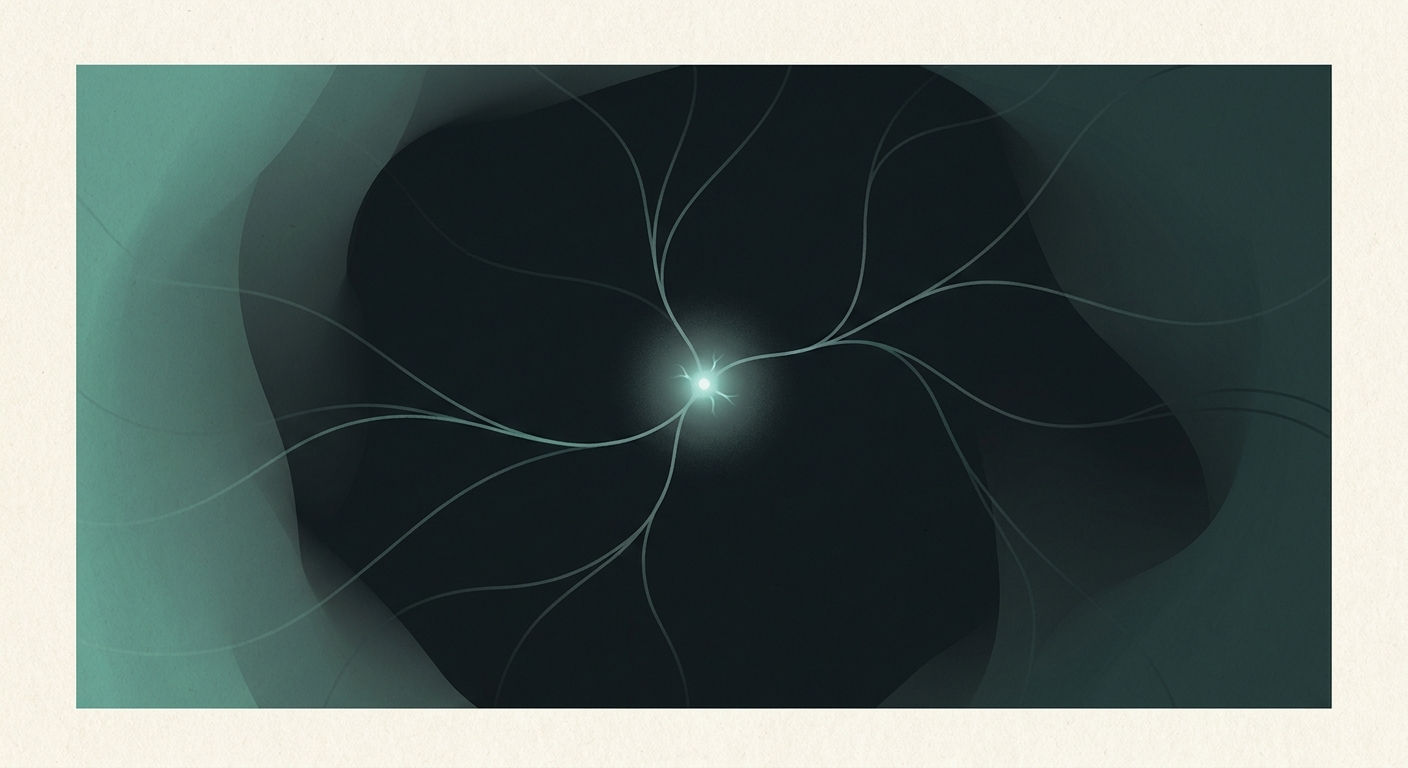
\includegraphics[width=0.42\textwidth]{figures/fig_spark.png}\\[4mm]
{\sffamily\bfseries\color{teal}\Large Now go build one.}\\[2mm]
{\sffamily\color{slate} github.com/VizuaraAI/pharma-slm \quad\textbullet\quad pharma-slm-vizuara.vercel.app}
\end{center}


\end{document}
